\section{Implementation of a SIPG Method}

In this section we mention the main problems arising at an implementation of a finite element method. A detailed survey can be also found in \cite[Section 0.6]{BS2002} and \cite[Chapter 8]{Braess2003}.
We assume that $\Omega$ is polygonal and we have a regular triangulation of $\Omega$ given. One main problem in the implementation of a SIPG method (or any finite element method) is the assembly of matrix defined by the left-hand side inner product. As suggest in the form in \eqref{eq:inner product SIPG} we evaluate the integrals on every triangle, edge respectively individually.

\subsection{Integration scheme}
First, to evaluate an integral numerically we need an integration scheme. Usually Gauss quadrature is the method of choice. To estimate the integral $\myIntX {\phantom{x}} {h(x)} $ a Gauss quadrature formula $\sum_{i=1}^{N} w_i h(q_i)$ needs to evaluate $h$ at certain quadrature points $q$. For the case $N=7$ we show the quadrature points for a triangular domain in figure \ref{fig: quadrature}.
\begin{figure}[!h]
	\centering
	
\usetikzlibrary{calc}

\newcommand{\baryc}[3]{  ($({ {#1}*\xOneRef + #2*\xTwoRef +#3*\xThreeRef}, 
                                                { {#1}*\yOneRef + #2*\yTwoRef +#3*\yThreeRef})$)  }

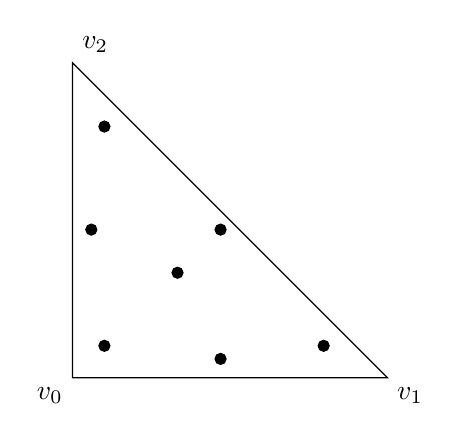
\begin{tikzpicture}[scale = 4,
]
	\def \xOneRef {0};
	\def \yOneRef {0};
	\def \xTwoRef {1};
	\def \yTwoRef {0};
	\def \xThreeRef {0};
	\def \yThreeRef {1};

	\coordinate (POneRef) at (\xOneRef, \yOneRef);
	\coordinate (PTwoRef) at (\xTwoRef, \yTwoRef);
	\coordinate (PThreeRef) at (\xThreeRef, \yThreeRef);


	\draw (0,0) -- (0,1) -- (1,0) -- cycle;

%draw point in ref triangle
	\draw[fill] (POneRef) circle (0.0pt) node [below left] {$v_0$};
	\draw[fill] (PTwoRef) circle (0.0pt)node [below right] {$v_1$};
	\draw[fill] (PThreeRef) circle (0.0pt)node [above right] {$v_2$};

	\def \a {0.470142};
	\def \b {0.0597159};
	\def \c {0.101287};
	\def \d {0.797427};
  	\draw[fill] \baryc {0.333333} {0.33333} {0.33333} circle (0.5pt);
  	\draw[fill] \baryc {\b} {\a} {\a} circle (0.5pt);
  	\draw[fill] \baryc {\a} {\b} {\a} circle (0.5pt);
 	\draw[fill] \baryc {\a} {\a} {\b} circle (0.5pt);
  	\draw[fill] \baryc {\d} {\c} {\c} circle (0.5pt);
  	\draw[fill] \baryc {\c} {\d} {\c} circle (0.5pt);
  	\draw[fill] \baryc {\c} {\c} {\d} circle (0.5pt);
\end{tikzpicture}
	\caption{Quadrature points for a integral over a triangle domain with $N=7$}
	 \label{fig: quadrature}
\end{figure}
Quadrature formulas, i.e. quadrature points and weights, especially for handling volume integrals can be found in \cite{Strout1971}.
To assemble the stiffness matrix $M$ the data we have to provide reduces to the data at the element, face respectively quadrature points.  
At an element quadrature point these are the gradients, whereas at a face quadrature point we need information about  the function values $u$ and the normal derivatives, i.e. $\nabla u \cdot \mathbf{n}$ of all test functions.

\subsection{A Reference Cell}
To reduce the storage space one usually specifies a reference cell $T_{ref}$ such that every triangle $T \in \triang$ is the image of $T_{ref}$ under an affine transformation $\Phi_T:T_{ref} \rightarrow T$. 
%We make use of the triangle spanned by the points $(0,0)^t, (0,1)^t$ and $(1,0)^t$ for our reference cell. 
Since the DG spaces also allow discontinuous functions a basis $p^1_{ref},\dots,p^n_{ref}$ of $T_{ref}$ also induces a basis on every $T$, namely the basis consisting of 
\[
	p_T^i(x) := p^i_{ref}(\Phi_T^{-1}(x)), \qquad x \in T, 1 \leq i \leq n.
\]
The most famous basis polynomials are the Lagrange elements, i.e. given a set of points $P$ each Lagrange basis element evaluate at exactly one point of $P$ to one and vanishes at every other point. Due to this property this basis is also referred as a nodal basis. 
A huge benefit of the Lagrange elements are their interpolation properties. 

Now most of the required data on a triangle $T$ can be easily derived knowing $\Phi_T$ and the reference cell $T_{ref}$. We explain how to do that in detail for the two-dimensional case.

\begin{example}\label{ex: base cell trafo}
From now an we consider $\Omega \subset \R^2$ and we choose the reference triangle to be the triangle spanned by the points $\point 0 0, \point 0 1$ and $\point 1 0$.
Suppose we want to figure out the transformation for the triangle $T = \langle v_1,v_2,v_3 \rangle$.
It has to hold
\[
\Phi\left(\point 0 0\right) = v_0, \Phi\left(\point 0 1\right) = v_1 \textnormal{ and } \Phi\left(\point 1 0\right) = v_2
\]
Since every two-dimensional affine transformation can be written in the form $\Phi(x) = Ax+b$ for some $A \in \R^{2 \times 2}$ and $b \in \R^2$ it is easy to verify that we have $A = \begin{pmatrix} v_1-v_0 & v_2-v_0\end{pmatrix}$ and $b = v_0$.
Having determined the transformation we are able to easily calculate its inverse $\Phi_T^{-1}(x) = A^{-1} (x-b) =: A^{-1} x- \tilde b$. \\
Let $\beta_0, \beta_1$ and $\beta_2$ be the barycentric coordinates of $x \in T$. Because of $\Phi^{-1}$'s linearity we find
\begin{align*}
	p^i_T(x) =& p_T^i( \beta_0 v_0 +\beta_1 v_1 + \beta_2 v_2  ) \\
	=& p^i_{ref}(\Phi_T^{-1}(\beta_0 v_0 +\beta_1 v_1 + \beta_2 v_2)) \\
	=& p^i_{ref}(\beta_0 \Phi_T^{-1}(v_0) +\beta_1 \Phi_T^{-1}(v_1) + \beta_2 \Phi_T^{-1}(v_2)) \\
		=& p^i_{ref}(\beta_0 \point 0 0 +\beta_1 \point 0 1 + \beta_2 \point 1 0 ), \qquad 1 \leq i \leq n.
\end{align*}
Thus, basis function values in $T$ can be simply determined by barycentric coordinates. Henceforth we refer with $x_{ref}$  to the point $\beta_0 \point 0 0 +\beta_1 \point 0 1 + \beta_2 \point 1 0$ which is the to $x$ corresponding point in the reference triangle . In Figure \ref{fig: transformation} the connection between $x_{ref}$ and $x$ is shown.

\begin{figure}[!h]
	
\usetikzlibrary{calc}
\usetikzlibrary{decorations.markings}
%\newcommand\fOne[2]{2*#1 + 0* #2 + 2}

%\fOne 1 1 

\begin{tikzpicture}[scale = 4,
]
	\def \xOneRef {0};
	\def \yOneRef {0};
	\def \xTwoRef {1};
	\def \yTwoRef {0};
	\def \xThreeRef {0};
	\def \yThreeRef {1};

	\coordinate (POneRef) at (\xOneRef, \yOneRef);
	\coordinate (PTwoRef) at (\xTwoRef, \yTwoRef);
	\coordinate (PThreeRef) at (\xThreeRef, \yThreeRef);

	\def \xRef {0.6};
	\def \yRef {0.2};
	\coordinate (PRef) at (\xRef, \yRef);


	\def \a {1.1};
	\def \b {0.4};
	\def \c {1.2};
	\def \d {0.3};

	\def \e {1.5};
	\def \f {0.5};

	\coordinate (xOneT) at ($({\a*\xOneRef+\b*\yOneRef+\e},{\c*\yOneRef+\d*\xOneRef+\f})$);
	\coordinate (xTwoT) at ($({\a*\xTwoRef+\b*\yTwoRef+\e},{\c*\yTwoRef+\d*\xTwoRef+\f})$);
	\coordinate (xThreeT) at ($({\a*\xThreeRef+\b*\yThreeRef+\e},{\c*\yThreeRef+\d*\xThreeRef+\f})$);

	\coordinate (xT) at ($({\a*\xRef+\b*\yRef+\e},{\c*\yRef+\d*\xRef+\f})$);


	\draw (0,0) -- (0,1) -- (1,0) -- cycle;
	\draw (xOneT) -- (xTwoT) -- (xThreeT) -- cycle;

%draw point in ref triangle
	\draw[fill] (POneRef) circle (0.6pt) node [below left] {$v^{ref}_0$};
	\draw[fill] (PTwoRef) circle (0.6pt)node [below right] {$v^{ref}_1$};
	\draw[fill] (PThreeRef) circle (0.6pt)node [above right] {$v^{ref}_2$};

	\draw[fill] (PRef) circle (0.6pt) node [left] {$x^{ref}$};


	\draw[fill] (xOneT) circle (0.6pt) node [left=0.1cm] {$v_0$};
	\draw[fill] (xTwoT) circle (0.6pt) node [right=0.2cm] {$v_1$};
	\draw[fill] (xThreeT) circle (0.6pt) node [above right] {$v_2$};

	\draw[fill] (xT) circle (0.6pt) node [left=0.1cm] {$\Phi(x^{ref}) =x$};

%	\draw[->, shorten >=0.5cm, shorten <=1cm] (PRef) edge [bend right] ($(xT)$);

	\draw[
			decoration = {markings, mark=at position 0.98 with {\arrow[scale=3, black]{stealth}}},
			postaction = {decorate},
			shorten >=5,
			shorten <=5,
			bend right] (PRef) to node [below] {{\Large $\Phi$}} ($(xT)-(0.005,0.005)$) ;

	%draw axes
	\draw[thick,->] (0, 0) -- (1.3,0);
	\draw[thick,->] (0, 0) -- (0,1.3);
	


\end{tikzpicture}
	\caption{Transformation of reference cell}
	 \label{fig: transformation}
\end{figure}

Similarly we can affiliate the determination of the gradient in $T$ to a calculation in $T_{ref}$. With the chain rule we have
\begin{align*}
	\left(\nabla_x p_T^i(x)\right)^t = D_x p_T^i(x) =& D_x p^i_{ref}(\Phi_T^{-1}(x)) \\
	  =& D_{\Phi_T^{-1}(x)}p^i_{ref}(\Phi_T^{-1}(x)) \cdot D_x  \Phi_T^{-1}(x) \\
	  =& D_{x_{ref}}p^i_{ref}(x_{ref}) \cdot  A^{-1}
\end{align*}
and thus
\begin{align}
	\nabla_x p_T^i(x) = A^{-t} \cdot \nabla_{x_{ref}}(x_{ref}), \qquad 1 \leq i \leq n. \label{eq: ref gradient}
\end{align}

Analogous proceeding yields for the Hessian matrix
\begin{align}
D_x^2p_T^i(x) = A^{-t} D_{x_{ref}}^2p^i_{ref}(x_{ref})  A^{-1}, \qquad 1 \leq i \leq n.
\end{align}

Concluding, if we need to determine function values, gradient and Hessian of a basis function on a cell, we only need the Jacobian of its transformation, i.e. $A$. We are able to calculate all further information with the data provided by the reference triangle.
\end{example}

\subsection{Refinement and Base Cells}\label{subsec: refinement and base cells}
Let us in the rest of this section further assume we have a triangulation of a two-dimensional domain $\Omega$. 
Suppose the mesh of our triangulation is created by refinement of a coarser mesh. We use a specific kind of refinement: Given a triangulation $\triang$ every triangle $T \in \triang$ is divided into four congruent triangles as is shown in figure \ref{pic: refinement}. We note, the finer grid $\triangFine$ for the diameter of each triangle is halved.

\begin{figure}[h]
\usetikzlibrary{calc}

		\begin{center}
		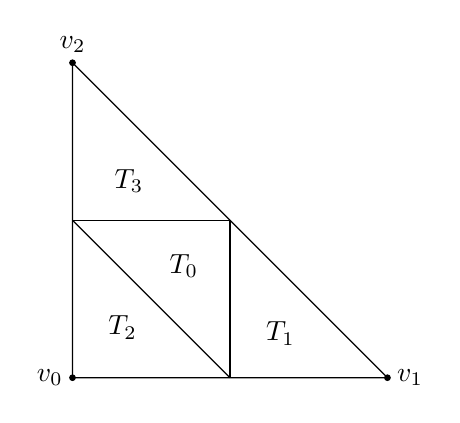
\begin{tikzpicture}
%define coordinates
			\coordinate (vEins) at (0,0) ;
			\coordinate (vZwei) at (0:4cm);
			\coordinate (vDrei) at (90:4cm);

%draw triangle
			\draw (vEins) -- (vZwei) -- (vDrei) -- cycle;

%draw refined triangle
			\draw ($(vEins)!0.5!(vZwei)$) -- ($(vEins)!0.5!(vDrei)$);
			\draw ($(vDrei)!0.5!(vZwei)$) -- ($(vEins)!0.5!(vDrei)$);
			\draw ($(vEins)!0.5!(vZwei)$) -- ($(vZwei)!0.5!(vDrei)$);

%draw nodes
			\draw[fill =black] (vEins) circle (1pt) node[left] {$ v_0$};
			\draw[fill =black] (vZwei) circle (1pt) node[right] {$v_1$};
			\draw[fill =black] (vDrei) circle (1pt) node[above] {$v_2$};

%			\draw node at (30:2.4cm) {$T_1$};

			\draw node at (45:0.9cm) {$T_2$};
			\draw node at (45:2cm) {$T_0$};
			\draw node at (74:2.6cm) {$T_3$};
			\draw node at (12:2.7cm) {$T_1$};

		\end{tikzpicture}
		\end{center}

\caption{Refinement of a triangle}
 \label{pic: refinement}
\end{figure}

We identify the new refined triangles with their original cell in $T$ calling it their basecell $T^T_b$. Repeating the refinement we can always relate a cell in the finest mesh with a basecell in the original triangulation. We can find an affine mapping $\Psi_T:T^T_b \rightarrow T$ transforming the $T^T_b$ to $T$ such that $\Phi_T = \Psi_T \circ \Phi_B$. This implies also that for the jacobians $A_{\Phi_T}, A_{\Psi_T}, A_{\Phi_B}$ of the affine transformations $\Phi_T, \Psi_T,\Phi_B$ holds
\begin{align}
A_{\Phi_T}=A_{\Psi_T} A_{\Phi_B}
\end{align} 

This makes saving information about the basecell very beneficial for the transformation matrix $A_{\Psi_T}$ is a diagonal matrix which even has the same entries along the diagonal. It even follows basis function data on two triangles with the same basecell only differ in a constant. Yet another benefit of the relation between cells and their basecells is they hav the same, or for the innermost triangle($T_0$ in figure \ref{pic: refinement}) opposite directed, normals.

\begin{example}\label{ex: leaf cell trafo}
In the two-dimensional case the Jacobian $A_{\Psi_T}$ of a transformation $\Psi_T$ from the base cell $B$ to a $l$ times refined triangle $T$ is $
	\begin{pmatrix}
		\frac 1 {2^l} & 0 \\ 0 & \frac 1 {2^l}
	\end{pmatrix} \text{ or }
	\begin{pmatrix}
		-\frac 1 {2^l} & 0 \\ 0 & -\frac 1 {2^l}
	\end{pmatrix}$, respectively if the number of intermediate basecells being an inner triangle during refinement  has been odd.

 To a point $x \in T$ we can determine a corresponding base cell point $x_B$, namely the point which satisfies $x = \Psi_T(x_B)$. With the help of \eqref{eq: ref gradient} we find the identity
\begin{align}
\nabla_x p_T^i(x) &= A_{\Phi_T}^{-t} \nabla_{x_{ref}} p^i_{ref} (x_{ref}) \nonumber\\
 &= A_{\Psi_T}^{-t} A_{\Phi_B}^{-t} \nabla_{x_{ref}} p^i_{ref} (x_{ref}) \nonumber\\
&= \epsilon 2^l A_{\Phi_B}^{-t} \nabla_{x_{ref}} p^i_{ref}(x_{ref}), \qquad \epsilon \in \{+,-\} \label{eq: trafo grad},
\end{align}
with $l \in \N$ indicating how often $T$ is refined with respect to the original mesh.\\
Analogously we have
\begin{align}
\nabla_x p^i(x) \mathbf n &= 2^l  A_{\Phi_B}^{-t} \cdot \nabla_{ref}p^i_{ref}(x_{ref}) \mathbf{ n_{b}} \qquad \text{ and } \label{eq: trafo normal der} \\
D_x^2 p^i(x) &= 2^{2l}  A_{\Phi_B}^{-t} D_{x_{ref}}^2 p^i_{ref}(x_{ref}), \qquad 1 \leq i \leq n,
\end{align}
where $\mathbf n_b$ is the to $n$ corresponding normal in the base cell. Note, that \eqref{eq: trafo normal der} even holds for inner refined triangles: The minus sign of the gradient cancels with the minus sign of the base cell normal $n_B$ since $n_B$ is opposite directed as the corresponding normal $n$ of a inner triangle.\\
Another case where the sign of the gradient \eqref{eq: trafo grad} could be important when we evaluate of the first part of the bilinearform, i.e. $\nabla \phi \cdot A \nabla v$. We first note, that two basis functions $p_T^i, p_T^j$ having only support on $T$ are created with the same affine mapping $\Phi_T$. Hence they have the same transposed, inversed Jacobian $A^{-t}_{\Phi_T}=\epsilon 2^l A_{\Phi_b}^{-t}$ and therefore the sign on the right-hand side in \eqref{eq: trafo grad} is for both gradients the same. Because we multiply both gradients a sign change between base and the actual cell does not affect the evaluation of our bilinear form. 
Of course for other combinations of basis polynomials the latter volume integral always equals zero because the polynomials' support is chosen in such a way that all other gradients vanish in the inner of $T$.

A usual error source are the signs of the terms
\[
	\jump {v \average{ A \nabla w }} = v^+ \frac 1 2  \left(A^+ \nabla w^+ + A^- \nabla w^-\right) \cdot \mathbf n^+ + v^- \frac 1 2 \left(A^+ \nabla w^+ + A^- \nabla w^-\right) \cdot \mathbf n^-.
\]
Since for two adjacent triangles always $\mathbf n^+ = - \mathbf n^-$ holds, we also have $A^+ \nabla w^+ \mathbf n^-= -A^+ \nabla w^+ \mathbf n^+$ and $A^- \nabla w^- \mathbf n^+= -A^- \nabla w^- \mathbf n^-$. Hence we can calculate the expression using \ref{eq: trafo normal der}. Note that all basic functions have support on only one triangle, such that for a evaluation of a basic functions $v_B$ either $v_B^+$ or $v_B^-$, just as for a basic functions $w_B$ either $w_B^+$ or $w_B^-$ equals to zero.

So, we are able to save a lot of memory if we store instead of all data at every quadrature points in each refined cell just the data of the base cell and the number of refinements. The refined cells contained in the actual mesh are referred as \emph{leaf cells}.
\end{example}

\subsection{Assembly Loop}
Another crux of the implementation is the handling of face terms, more specific: We mentioned earlier that we evaluate the bilinearform cell-wise. Hence the volume integrals are calculated visiting every cell only once. When do we compute the edge integrals?\\
Face terms can be collected either by assemble them in two steps or a more complex one.
For the two step variant the face terms are split up into the contributions of their two adjacent cells, such that the first part is assembled when processing the first adjacent cell and the second during the processing of the other adjacent cell. \\
In the one step variant we handle a face term when visiting an adjacent cell for first time. To detect the first time we introduce a cell flag for every leaf cell indicating whether the cell has been processed yet. Now, each time the assembling algorithm visits a face it determines the neighbouring cell and checks if the face has already been processed. The following algorithm \ref{alg: assembling} from \cite{BMV2009} illustrates how to perform this one step approach. 
\begin{algorithm}[H]
\caption{An assembling loop for a DG method}
\label{alg: assembling}
\begin{algorithmic}
\Ensure every cell flag is false
\For {cell in all leaf cells}  
\State get cell data
\State assemble volume integrals 
	\For {face in faces(cell)}
		\If {neighbour across the face exists} 
			\If {not neighbour flag}
					\State get neighbour cell data
					\State assemble face terms
			\EndIf
		\Else
			\State assemble boundary terms
		\EndIf
\EndFor
	\State cell flag to true 
\EndFor
\State Reset every cell flag to false
\end{algorithmic}
\end{algorithm}

In \cite{BMV2009} Brix et. alter also develop a data structure efficiently handling all the mentioned requirements among a lot of other features. On this structure our implementation used for the later numerical results is based on.